%2multibyte Version: 5.50.0.2953 CodePage: 1252
% green
% blue
% orange
% purple
% red
% resets numbering each section

\ifdefined\extendedversion\else
  \PassOptionsToClass{handout}{beamer}
\fi
\documentclass[xcolor=x11names,compress,aspectratio=169]{beamer}%
\usepackage{amsmath}
\usepackage{amsfonts}
\usepackage{amssymb}
\usepackage{graphicx}
\usepackage{tikz}
\usepackage{dcolumn}%
\setcounter{MaxMatrixCols}{30}
%TCIDATA{OutputFilter=latex2.dll}
%TCIDATA{Version=5.50.0.2953}
%TCIDATA{Codepage=1252}
%TCIDATA{CSTFile=beamer.cst}
%TCIDATA{Created=Monday, May 13, 2013 15:44:12}
%TCIDATA{LastRevised=Tuesday, October 07, 2025 12:58:59}
%TCIDATA{<META NAME="GraphicsSave" CONTENT="32">}
%TCIDATA{<META NAME="SaveForMode" CONTENT="1">}
%TCIDATA{BibliographyScheme=Manual}
%TCIDATA{<META NAME="DocumentShell" CONTENT="Other Documents\SW\Slides - Beamer">}
%TCIDATA{Language=American English}
%BeginMSIPreambleData
\providecommand{\U}[1]{\protect\rule{.1in}{.1in}}
%EndMSIPreambleData
%\usepackage{etex} %vers l'infini et au-dela
\usepackage{minted}
\beamertemplatenavigationsymbolsempty
\usepackage[utf8]{inputenc} 
\usepackage[T1]{fontenc} % pour taper les lettres accentuees
%\usepackage[francais, english]{babel} %le rapport est en franÁais 
\usepackage{amsthm,amssymb,amsbsy,amsmath,amsfonts,amscd,mathrsfs}
\usepackage{geometry} %pour la modification des marges
%\usepackage{fancyhdr} %pour modification des pieds de page
%\usepackage{lastpage} %numero de la derniËre page
\usepackage{lmodern}
\usepackage{lscape} % Pour pouvoir activer le mode landscape
\usepackage{booktabs} %tableaux
\usepackage{float}	%pour forcer le placement des images.
\usepackage{graphicx} %pour afficher des images
\usepackage{longtable} %tables sur plusieurs pages
\usepackage{animate} %transformer des gifs
\usepackage{caption}
\captionsetup{labelformat=simple}
\setbeamertemplate{caption}[numbered]
\setbeamerfont{caption}{size=\scriptsize}
\usepackage[scriptsize]{subfigure}
\usepackage{multirow} 			%fusionner lignes
\usepackage{tikz}
\usepackage{adjustbox}
\usetikzlibrary{arrows,positioning}
\usetikzlibrary{mindmap,trees,shadows,backgrounds}
\usepackage{tabularx}
\usepackage{verbatim}%insertion de code
\usepackage{listings}
\usepackage{dsfont} % Pour les lettres mathematiques
\usepackage{hyperref} %pour que les references soient des liens hypertextes
\usepackage{natbib}
\usepackage{bibentry}
\usepackage{color}
\definecolor{bg}{rgb}{0.95,0.95,0.95}

\def\LECTURENAME{Mod\'elisation, estimation, simulation des risques climatiques}
\def\DIPLOMA{Master in Economics, 2$^{nd}$ year}
\def\UNIV{Ecole Polytechnique}
\def\WEBPAGE{\href{http://vermandel.fr/btm/}{http://vermandel.fr/btm}}
\def\SHORTNAME{Modélisation, estimation, simulation des risques climatiques}



%\usepackage{mathpazo}
\usepackage{multimedia}
\usepackage{dcolumn}
\usepackage{mathtools}
\usepackage{xspace}
\usepackage{array}%

\usepackage{graphicx}

\definecolor{light-gray}{gray}{0.85}
\usepackage{ragged2e} % Pour justifier
\definecolor{bleu}{RGB}{0,129,188}
\definecolor{rouge}{RGB}{238,50,78}
\definecolor{orange}{RGB}{255,100,0}
\definecolor{vert}{RGB}{0,157,87}
\newtheorem{hypothese}{Hypoth\`ese}
\newtheorem{remarque}{Hypoth\`ese}
\newtheorem{theoreme}{Th\'eor\`eme}[section]
\newtheorem{definitionDeux}{D\'efinition}[section]
\newcommand{\iid}{\stackrel{\mathrm{iid}}{\sim}}
\usepackage[official,right]{eurosym} % symbols euro
\usepackage{gensymb} % symbole degre \degre
\usepackage{eurosym} % symbole euro
\usepackage{rotating}
\usepackage{multicol}

% Bibliographie
%\usepackage{bib entry}
%\nobibliography*
%\let\newblock\relax

%\usepackage[notocbib]{apacite}
%\usepackage[style=apa]{biblatex}
%\usepackage[round]{natbib}
%\usepackage[style=authoryear]{biblatex}
%\usepackage[backend=bibtex, style=authoryear-comp]{biblatex}
%\usepackage{biblatex}
%\renewcommand*{\bibfont}{\scriptsize} % Pour avoir la biblio en plus petit
%\usepackage{apacite}
%\bibliographystyle{apacite}

\justifying %on justifie le texte du document
\definecolor{deepblue}{RGB}{0,129,188}
\definecolor{deepblue2}{RGB}{158, 64, 57}
\definecolor{deepblue3}{RGB}{245, 84, 66}


% Pour l'annexe (http://tex.stackexchange.com/questions/2541/beamer-frame-numbering-in-appendix)
\newcommand{\backupbegin}{
   \newcounter{framenumberappendix}
   \setcounter{framenumberappendix}{\value{framenumber}}
}
\newcommand{\backupend}{
   \addtocounter{framenumberappendix}{-\value{framenumber}}
   \addtocounter{framenumber}{\value{framenumberappendix}} 
}

%\usepackage{epstopdf}
%\epstopdfDeclareGraphicsRule{.gif}{png}{.png}{%
%  convert gif:#1 png:\OutputFile
%}
%\AppendGraphicsExtensions{.gif}

% A NE PAS UTILISER !
%\let\olditem=\item% 
%\renewcommand{\item}{\olditem \justifying}%

\justifying

%\graphicspath{{../images}}


\usepackage{dcolumn}


% THEME %
\usetheme{Frankfurt}
\useoutertheme[subsection=false,shadow]{miniframes}

\addtobeamertemplate{background canvas}{\transfade[duration=.3]}{}

% Fonts
%\usefonttheme[onlymath]{serif}
%\usefonttheme{structuresmallcapsserif}
%\usefonttheme[onlymath]{mathserif}
%\usefonttheme{serif}
\setbeamerfont{section in head/foot}{size=\tiny, shape=\normalfont}
\setbeamerfont{subsection in toc}{shape=\normalfont, size = \scriptsize}
\setbeamerfont{section in toc}{size = \small, shape=\normalfont}
% Colours
\setbeamercolor{section in head/foot}{fg=black, bg=gray!5}
\setbeamercolor{frametitle}{bg=white, fg=black}
\setbeamercolor{lower separation line head}{bg=black!5}

\setbeamertemplate{sections/subsections in toc}[square]
\setbeamertemplate{items}[triangle]
\setbeamertemplate{itemize subitem}[triangle]
\setbeamertemplate{itemize subsubitem}[ball]
\setbeamertemplate{enumerate items}[default]
\setbeamertemplate{frametitle}[default][rounded=false,shadow=true]

\setbeamercovered{transparent}



\usepackage{assets/beamerouterthemeEwen}
\usepackage{assets/beamercolorthemeEwen}
\usepackage{assets/beamerhighlight}


\newcommand*\grasO[1]{\textbf{\textcolor{orange}{#1}}} 
\newcommand*\grasR[1]{\textbf{\textcolor{rouge}{#1}}}
\newcommand*\grasV[1]{\textbf{\textcolor{vert}{#1}}} 
\newcommand*\grasB[1]{\textbf{\textcolor{bleu}{#1}}} 


\definecolor{rcp26}{RGB}{39, 55, 122}
\definecolor{rcp45}{RGB}{112, 159, 200}
\definecolor{rcp60}{RGB}{222, 99, 43}
\definecolor{rcp85}{RGB}{205, 16, 32}
\definecolor{dp}{RGB}{181, 73, 60}

\newcommand*\grasRCPa[1]{\textbf{\textcolor{rcp26}{#1}}}
\newcommand*\grasRCPb[1]{\textbf{\textcolor{rcp45}{#1}}} 
\newcommand*\grasRCPc[1]{\textbf{\textcolor{rcp60}{#1}}} 
\newcommand*\grasRCPd[1]{\textbf{\textcolor{rcp85}{#1}}} 
%\newcommand {\red} {\color{red}}
\newcommand {\white} {\color{white}}
%\newcommand {\black} {\color{black}}
\def\Frac#1#2{ #1 \color{red}\above 0.4pt \normalcolor #2}


\usetikzlibrary{decorations}
\usetikzlibrary{decorations.pathmorphing}
\usetikzlibrary{shapes.geometric}
\usetikzlibrary{calc}
\usetikzlibrary{decorations.fractals}
\useoutertheme[subsection=false,shadow]{miniframes}
\useinnertheme{default}
\usefonttheme{serif}
\setbeamerfont{title like}{shape=\scshape}
\setbeamerfont{frametitle}{shape=\scshape}
\setbeamercolor*{lower separation line head}{bg=DeepSkyBlue4}
\setbeamercolor*{normal text}{fg=black,bg=white}
\setbeamercolor*{alerted text}{fg=dp}
\setbeamercolor*{example text}{fg=black}
\setbeamercolor*{structure}{fg=black}
\setbeamercolor*{palette tertiary}{fg=black,bg=black!10}
\setbeamercolor*{palette quaternary}{fg=black,bg=black!10}
\renewcommand{\(}{\begin{columns}}
\renewcommand{\)}{\end{columns}}
\newcommand{\<}[1]{\begin{column}{#1}}
\renewcommand{\>}{\end{column}}
\setbeamertemplate{navigation symbols}{}
\setbeamertemplate{headline}{}
\setbeamertemplate{footline}
{
\leavevmode
\hbox{\begin{beamercolorbox}[wd=1\paperwidth,ht=2.25ex,dp=1ex,center]{title in head/foot}\usebeamerfont{title in head/foot}\hfill\hspace*{12em}\insertshorttitle\hspace*{3em}
\insertframenumber{} / \inserttotalframenumber\hspace*{1ex}
\end{beamercolorbox}}
\vskip0pt
}
\newcommand {\red} {\color{red}}
\newcommand {\black} {\color{black}}
\newcommand{\green}{\color{green}}
\definecolor{deepblue}{RGB}{0,129,188}
\newcommand{\pink}{\color{magenta}}
\newcommand{\blue}{\color{deepblue}}
\hypersetup{
colorlinks = true,citecolor=deepblue3,linkcolor=deepblue2
}
\setbeamercolor{frametitle}{fg=deepblue2,bg=white}
\makeatletter
\AtBeginSection[]
{
\ifnum \value{framenumber}>2
\begin{frame}<beamer>
\frametitle{Plan}
\tableofcontents[currentsection,subsectionstyle=hide]
\end{frame}
\else
\fi
}
\let\oldtextbf\textbf
\renewcommand{\textbf}[1]{\textcolor{dp}{\oldtextbf{#1}}}
\newcommand*\annotatedFigureBoxGOT[2]{\draw[thick,rounded corners,deepblue2] (#1) rectangle (#2);}
\newcommand*\annotatedFigureBoxARR[2]{\draw[->,thick,rounded corners,deepblue2] (#1) -- (#2);}
\newcommand*\annotatedFigureBoxCustom[8]{\draw[#5,thick,rounded corners] (#1) rectangle (#2);\node at (#4) [fill=#6,thick,shape=circle,draw=#7,inner sep=2pt,font=\sffamily,text=#8] {\textbf{#3}};}
\newcommand*\annotatedFigureBox[4]{\annotatedFigureBoxCustom{#1}{#2}{#3}{#4}{deepblue2}{deepblue2}{black}{black}}
\newcommand*\annotatedFigureText[4]{\node[draw=none, anchor=south west, text=#2, inner sep=0, text width=#3\linewidth,font=\sffamily] at (#1){#4};}
\newenvironment {annotatedFigure}[1]{\centering\begin{tikzpicture}
\node[anchor=south west,inner sep=0] (image) at (0,0) { #1};\begin{scope}[x={(image.south east)},y={(image.north west)}]}{\end{scope}\end{tikzpicture}}

\usetheme[numbering=none,progressbar=frametitle]{metropolis}
\setbeamertemplate{footline}{
\hfill\usebeamerfont{page number in head/foot}\insertpagenumber/\insertpresentationendpage\hspace{1em}
}
\usetikzlibrary{arrows.meta, positioning, shapes.misc, fit}
\newenvironment{stepenumerate}{\begin{enumerate}[<+->]}{\end{enumerate}}
\newenvironment{stepitemize}{\begin{itemize}[<+->]}{\end{itemize} }
\newenvironment{stepenumeratewithalert}{\begin{enumerate}[<+-| alert@+>]}{\end{enumerate}}
\newenvironment{stepitemizewithalert}{\begin{itemize}[<+-| alert@+>]}{\end{itemize} }
\newtheorem{assumption}[theorem]{Assumption}
\setlength{\itemsep}{1em}
\definecolor{ssp1}{RGB}{27,158,119}
\definecolor{ssp2}{RGB}{55,126,184}
\definecolor{ssp3}{RGB}{217,95,2}
\definecolor{ssp4}{RGB}{152,78,163}
\definecolor{ssp5}{RGB}{228,26,28}
\newcommand{\ssponebullet}{\textcolor[RGB]{27,158,119}{\large\textbullet}}
\newcommand{\ssptwobullet}{\textcolor[RGB]{55,126,184}{\large\textbullet}}
\newcommand{\sspthreebullet}{\textcolor[RGB]{217,95,2}{\large\textbullet}}
\newcommand{\sspfourbullet}{\textcolor[RGB]{152,78,163}{\large\textbullet}}
\newcommand{\sspfivebullet}{\textcolor[RGB]{228,26,28}{\large\textbullet}}
\definecolor{forc19}{RGB}{255,230,230}
\definecolor{forc26}{RGB}{255,180,180}
\definecolor{forc45}{RGB}{255,120,120}
\definecolor{forc70}{RGB}{220,50,50}
\definecolor{forc85}{RGB}{150,0,0}
% Compact is the default: each item list is static.
% The extended wrapper turns lists into progressive overlays for lecture delivery.
\ifdefined\extendedversion
  \let\compactitemize\itemize
  \let\endcompactitemize\enditemize
  \renewenvironment{itemize}{\begin{compactitemize}[<+-| alert@+>]}{\end{compactitemize}}
  \renewenvironment{stepitemize}{\begin{compactitemize}[<+->]}{\end{compactitemize}}
  \renewenvironment{stepitemizewithalert}{\begin{compactitemize}[<+-| alert@+>]}{\end{compactitemize}}
\else
  % Static handout: all list content is fully visible, with no animation fade.
  \renewenvironment{stepitemize}{\begin{itemize}}{\end{itemize}}
  \renewenvironment{stepitemizewithalert}{\begin{itemize}}{\end{itemize}}
  \renewenvironment{stepenumerate}{\begin{enumerate}}{\end{enumerate}}
  \renewenvironment{stepenumeratewithalert}{\begin{enumerate}}{\end{enumerate}}
  \setbeamercovered{transparent=100}
\fi
\begin{document}
%

%TCIMACRO{\TeXButton{GG}{\title[\SHORTNAME]{
%\textsc{\footnotesize\SHORTNAME\\ Session 3\\[0.35em] \Large
%Scenario building of Integrated Assessment Models}
%\\
%}
%\author{ Gauthier Vermandel\\
%{\footnotesize Ecole polytechnique}}
%\date{}}}%
%BeginExpansion
\title[\SHORTNAME]{
\textsc{\footnotesize\SHORTNAME\\ Session 3\\[0.35em] \Large
Scenario building of Integrated Assessment Models}
\\
}
\author{ Gauthier Vermandel\\
{\footnotesize Ecole polytechnique}}
\date{}%
%EndExpansion
%

%TCIMACRO{\TeXButton{BeginFrame}{\begin{frame}}}%
%BeginExpansion
\begin{frame}%
%EndExpansion
%

%TCIMACRO{\TeXButton{\maketitle}{\maketitle}}%
%BeginExpansion
\maketitle
%EndExpansion
%

%TCIMACRO{\TeXButton{Transition: Box Out}{\transboxout}}%
%BeginExpansion
\transboxout
%EndExpansion%
%TCIMACRO{\TeXButton{EndFrame}{\end{frame}}}%
%BeginExpansion
\end{frame}%
%EndExpansion
%

%TCIMACRO{\TeXButton{BeginFrame}{\begin{frame}}}%
%BeginExpansion
\begin{frame}%
%EndExpansion
%

%TCIMACRO{\QTR{frametitle}{Schedule of the day}}%
%BeginExpansion
\frametitle{Schedule of the day}%
%EndExpansion


\textbf{Objectives}

\begin{itemize}
\item Understanding the \textbf{basics} of \textbf{Integrated Assessment
Models}.

\item Build and \textbf{simulating macro-climate scenarios} using IPCC\ and
NGFS\ methodology.%
%TCIMACRO{\TeXButton{vspace}{\vspace{1ex}}}%
%BeginExpansion
\vspace{1ex}%
%EndExpansion

\end{itemize}

\textbf{Materials:}

\begin{itemize}
\item \textsf{notebook\_session3.ipynb} \textit{notebook introduction
of model's options.}

\item \textsf{notebook\_session3.ipynb} \textit{notebook
exercises about scenarii simulations.}

\item \textsf{Handout\_DICE.pdf} a synthetic presentation of the DICE\ model.
\end{itemize}

%

%TCIMACRO{\TeXButton{Transition: Box Out}{\transboxout}}%
%BeginExpansion
\transboxout
%EndExpansion%
%TCIMACRO{\TeXButton{EndFrame}{\end{frame}}}%
%BeginExpansion
\end{frame}%
%EndExpansion


\section{Introduction}%

%TCIMACRO{\TeXButton{BeginFrame}{\begin{frame}}}%
%BeginExpansion
\begin{frame}%
%EndExpansion
%

%TCIMACRO{\QTR{frametitle}{Introduction: why IAMs matter for policy and
%finance}}%
%BeginExpansion
\frametitle{Introduction: why IAMs matter for policy and finance}%
%EndExpansion


\begin{center}
\begin{tikzpicture}[
box/.style={rounded corners=2pt, line width=0.5pt,
  text width=4.65cm, minimum height=1.05cm, inner sep=7pt,
  align=center, font=\small},
econ/.style={box, draw=blue!25!gray, fill=blue!4},
energy/.style={box, draw=teal!40!gray, fill=teal!5},
emit/.style={box, draw=orange!45!gray, fill=orange!6},
clim/.style={box, draw=red!30!gray, fill=red!4},
policy/.style={box, draw=teal!45!gray, fill=teal!5},
arr/.style={-{Latex[length=2mm,width=1.4mm]}, line width=0.65pt, draw=black!60},
polarr/.style={arr, draw=teal!75!black},
damarr/.style={arr, draw=red!65!black},
labeltext/.style={font=\scriptsize, fill=white, inner sep=2pt}
]
% Same two-column structure; restrained fills and consistent typography.
\node[econ] (drivers) at (0,0) {\textbf{Socioeconomic drivers}\\[2pt]
  \footnotesize Population $L_t$, TFP $A_t$, \ldots};
\node[econ] (economy) at (0,-1.85) {\textbf{Economy}\\[2pt]
  \footnotesize Output $Y_t$, capital $K_t$, \ldots};
\node[policy] (policy) at (0,-3.7) {\textbf{Policy instruments}\\[2pt]
  \footnotesize Carbon price $\tau_t$, abatement $\mu_t$};
\node[energy] (system) at (8,0) {\textbf{Energy \& land system}\\[2pt]
  \footnotesize Tech mix, intensity $\sigma_t$};
\node[emit] (emiss) at (8,-1.85) {\textbf{Emissions} $E_t$\\[2pt]
  \footnotesize Fossil + land-use};
\node[clim] (climate) at (8,-3.7) {\textbf{Climate system}\\[2pt]
  \footnotesize Carbon cycle + temperature $T_t$};
% Main causal links.
\draw[arr] (drivers.south) -- (economy.north);
\draw[arr] (system.south) -- (emiss.north);
\draw[arr] (economy.east) -- (emiss.west);
\draw[arr] (emiss.south) -- node[labeltext,right=3pt]{GHGs} (climate.north);
\draw[polarr] (policy.north) -- (economy.south);
% Separate lanes: policy enters emissions below the main horizontal link;
% climate damages return to the economy through the inter-row corridor.
\draw[polarr, rounded corners=5pt]
  (policy.east) -- (4.5,-3.7) -- (4.5,-2.15)
  -- node[labeltext,below=1pt,text=teal!75!black]{Abatement $\mu_t$}
  ([yshift=-0.3cm]emiss.west);
\draw[damarr, rounded corners=5pt]
  ([xshift=-1.5cm]climate.north) -- (6.5,-2.8) -- (1.5,-2.8)
  -- ([xshift=1.5cm]economy.south);
\node[labeltext,text=red!65!black] at (2.8,-2.8) {Climate damages};
\end{tikzpicture}



\end{center}

%

%TCIMACRO{\TeXButton{Transition: Box Out}{\transboxout}}%
%BeginExpansion
\transboxout
%EndExpansion%
%TCIMACRO{\TeXButton{EndFrame}{\end{frame}}}%
%BeginExpansion
\end{frame}%
%EndExpansion
%

%TCIMACRO{\TeXButton{BeginFrame}{\begin{frame}}}%
%BeginExpansion
\begin{frame}%
%EndExpansion
%

%TCIMACRO{\QTR{frametitle}{Introduction: IAMs in practice: NGFS Scenarios}}%
%BeginExpansion
\frametitle{Introduction: IAMs in practice: NGFS Scenarios}%
%EndExpansion


\begin{itemize}
\item IAMs provide scenario pathways $\Rightarrow$

\begin{itemize}
\item \textbf{Temperature evolution} under different policies.

\item \textbf{Physical risk impacts}: GDP losses from climate damages.

\item \textbf{Transition risk impacts}: carbon price trajectories.
\end{itemize}

\item Used for \textbf{stress-testing} and \textbf{risk assessment} in finance.
\end{itemize}

\centering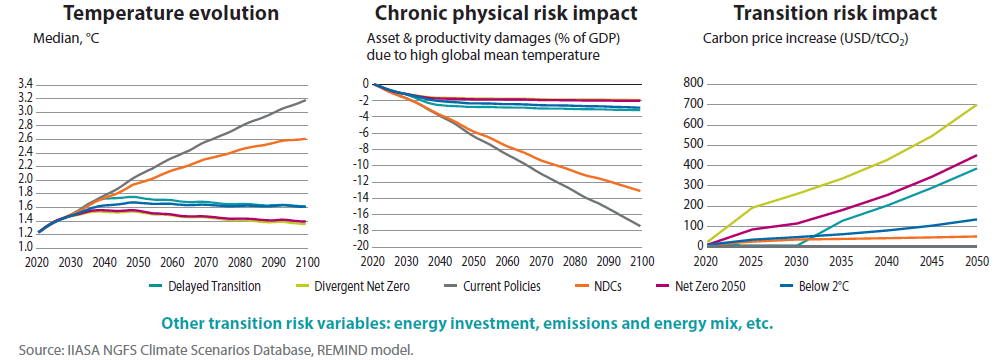
\includegraphics[width=0.7\linewidth]{images/NGFS.png}

{\scriptsize NGFS = Network for Greening the Financial System (central banks
and supervisors).}%

%TCIMACRO{\TeXButton{Transition: Box Out}{\transboxout}}%
%BeginExpansion
\transboxout
%EndExpansion%
%TCIMACRO{\TeXButton{EndFrame}{\end{frame}}}%
%BeginExpansion
\end{frame}%
%EndExpansion
%

%TCIMACRO{\TeXButton{BeginFrame}{\begin{frame}}}%
%BeginExpansion
\begin{frame}%
%EndExpansion
%

%TCIMACRO{\QTR{frametitle}{Introduction: why IAMs matter for policy and
%finance}}%
%BeginExpansion
\frametitle{Introduction: why IAMs matter for policy and finance}%
%EndExpansion


\begin{itemize}
\item \textbf{For financial institutions:}

\begin{itemize}
\item IAM outputs (e.g. from NGFS scenarios) are used by central banks and
supervisors for \textbf{climate stress-testing exercises}.

\item Provide pathways for GDP, energy, emissions, and damages under different policies.
\end{itemize}

\item \textbf{For international policy:}

\begin{itemize}
\item IAMs feed into \textbf{IPCC reports}, underpinning assessments of
mitigation costs and impacts.

\item Establish a common reference for climate policy design across countries.
\end{itemize}

\item \textbf{For carbon pricing:}

\begin{itemize}
\item Benchmark for the \textbf{social cost of carbon}.

\item Example: the US administration (Biden) adopted \$52/ton
CO\textsubscript{2} based on IAM results (incl. DICE).
\end{itemize}
\end{itemize}

%

%TCIMACRO{\TeXButton{Transition: Box Out}{\transboxout}}%
%BeginExpansion
\transboxout
%EndExpansion%
%TCIMACRO{\TeXButton{EndFrame}{\end{frame}}}%
%BeginExpansion
\end{frame}%
%EndExpansion
%

%TCIMACRO{\TeXButton{BeginFrame}{\begin{frame}}}%
%BeginExpansion
\begin{frame}%
%EndExpansion
%

%TCIMACRO{\QTR{frametitle}{Introduction: Why do we have a variety of
%scenarios?}}%
%BeginExpansion
\frametitle{Introduction: Why do we have a variety of scenarios?}%
%EndExpansion


\begin{itemize}
\item Climate scenarios are not forecasts: they are \textbf{``what if''}
explorations. \vspace{0.5em}

\item They differ because of two main ingredients:%
%TCIMACRO{\TeXButton{vspace}{\vspace{1ex}}}%
%BeginExpansion
\vspace{1ex}%
%EndExpansion


\begin{enumerate}
\item \textbf{Socioeconomic narratives (SSPs)}

\begin{itemize}
\item Long-run assumptions on population, economic growth, inequality.

\item Energy and land-use technology adoption (renewables, CCS, etc.).

\item Speed of structural change and decarbonization potential.
\end{itemize}

\item \textbf{Policy implementation (forcing levels)}

\begin{itemize}
\item Presence (or absence) of a carbon price.

\item How fast the carbon tax rises over time.

\item Coverage: local vs. global implementation, uniform vs. fragmented.
\end{itemize}
\end{enumerate}

\vspace{0.8em}

\item \textbf{Together, narratives + policy assumptions build the SSP scenario
matrix used by the IPCC.}
\end{itemize}

%

%TCIMACRO{\TeXButton{Transition: Box Out}{\transboxout}}%
%BeginExpansion
\transboxout
%EndExpansion%
%TCIMACRO{\TeXButton{EndFrame}{\end{frame}}}%
%BeginExpansion
\end{frame}%
%EndExpansion
%

%TCIMACRO{\TeXButton{BeginFrame}{\begin{frame}}}%
%BeginExpansion
\begin{frame}%
%EndExpansion
%

%TCIMACRO{\QTR{frametitle}{Introduction: roadmap for today}}%
%BeginExpansion
\frametitle{Introduction: roadmap for today}%
%EndExpansion


\begin{itemize}
\item Explain the role of \textbf{Integrated Assessment Models (IAMs)} in
climate-economy analysis. \vspace{0.5em}

\item Learn how climate scenarios are \textbf{constructed}, not predicted:

\begin{itemize}
\item \textbf{Narrative dimension}: socioeconomic pathways (SSPs), growth,
technology, demographics.

\item \textbf{Policy dimension}: climate policy ambition (carbon pricing,
mitigation targets).
\end{itemize}

\vspace{0.5em}

\item Understand the \textbf{IPCC scenario matrix} (SSP - forcing levels) and
its role in assessments (e.g. CMIP6). \vspace{0.5em}

\item Explore the DICE model as a \textbf{case study}: its building blocks,
trade-offs, and illustrative simulations.
\end{itemize}

%

%TCIMACRO{\TeXButton{Transition: Box Out}{\transboxout}}%
%BeginExpansion
\transboxout
%EndExpansion%
%TCIMACRO{\TeXButton{EndFrame}{\end{frame}}}%
%BeginExpansion
\end{frame}%
%EndExpansion
%

%TCIMACRO{\TeXButton{BeginFrame}{\begin{frame}}}%
%BeginExpansion
\begin{frame}%
%EndExpansion
%

%TCIMACRO{\QTR{frametitle}{Introduction: where does DICE fit in this
%landscape?}}%
%BeginExpansion
\frametitle{Introduction: where does DICE fit in this landscape?}%
%EndExpansion


\begin{itemize}
\item \textbf{Strength}: standard economic block + climate module (carbon
cycle, temperatures) $\Rightarrow$ clear insight into mechanisms and the
\emph{social cost of carbon}.%
%TCIMACRO{\TeXButton{vspace}{\vspace{2ex}}}%
%BeginExpansion
\vspace{2ex}%
%EndExpansion


\item \textbf{Limits}: no sectoral detail, no fine multi-regional structure,
limited uncertainty $\Rightarrow$ complement to complex IAMs.%
%TCIMACRO{\TeXButton{vspace}{\vspace{2ex}}}%
%BeginExpansion
\vspace{2ex}%
%EndExpansion


\item \textbf{Use}: conceptual benchmark, teaching tool, stress-testing
policies, part of the five core models used by Biden's administration to set
the carbon price (\$52/ton carbon).
\end{itemize}

%

%TCIMACRO{\TeXButton{Transition: Box Out}{\transboxout}}%
%BeginExpansion
\transboxout
%EndExpansion%
%TCIMACRO{\TeXButton{EndFrame}{\end{frame}}}%
%BeginExpansion
\end{frame}%
%EndExpansion
%

%TCIMACRO{\TeXButton{PAPER OUTLINE}{\begin{frame}{Outline}
%\tableofcontents\end{frame}}}%
%BeginExpansion
\begin{frame}{Outline}
\tableofcontents\end{frame}%
%EndExpansion


\section{Shared Socioeconomic Pathways (SSPs)}%

%TCIMACRO{\TeXButton{BeginFrame}{\begin{frame}}}%
%BeginExpansion
\begin{frame}%
%EndExpansion
%

%TCIMACRO{\QTR{frametitle}{SSPs: Key definitions}}%
%BeginExpansion
\frametitle{SSPs: Key definitions}%
%EndExpansion


\begin{itemize}
\item \textbf{SSPs (Shared Socioeconomic Pathways):} Narratives + quantitative
pathways describing alternative futures of population, GDP, technology, land
use, energy.%
%TCIMACRO{\TeXButton{vspace}{\vspace{2ex}}}%
%BeginExpansion
\vspace{2ex}%
%EndExpansion


\item \textbf{CMIP (Coupled Model Intercomparison Project):} International
framework where Earth System Models (ESMs) simulate climate under common
scenarios.%
%TCIMACRO{\TeXButton{vspace}{\vspace{2ex}}}%
%BeginExpansion
\vspace{2ex}%
%EndExpansion


\item \textbf{IPCC:} Not a research body itself. It \emph{assesses} the
scientific literature (incl. IAMs \& CMIP runs) to produce consensus reports.
\end{itemize}

%

%TCIMACRO{\TeXButton{Transition: Box Out}{\transboxout}}%
%BeginExpansion
\transboxout
%EndExpansion%
%TCIMACRO{\TeXButton{EndFrame}{\end{frame}}}%
%BeginExpansion
\end{frame}%
%EndExpansion
%

%TCIMACRO{\TeXButton{BeginFrame}{\begin{frame}}}%
%BeginExpansion
\begin{frame}%
%EndExpansion
%

%TCIMACRO{\QTR{frametitle}{SSPs: Why Shared Socioeconomic Pathways (SSPs)?}}%
%BeginExpansion
\frametitle{SSPs: Why Shared Socioeconomic Pathways (SSPs)?}%
%EndExpansion


\begin{itemize}
\item Provide a \textbf{common framework} for socio-economic and climate
futures.%
%TCIMACRO{\TeXButton{vspace}{\vspace{2ex}}}%
%BeginExpansion
\vspace{2ex}%
%EndExpansion


\item Two building blocks:%
%TCIMACRO{\TeXButton{vspace}{\vspace{1ex}}}%
%BeginExpansion
\vspace{1ex}%
%EndExpansion


\begin{enumerate}
\item \textbf{Narratives (qualitative)}: governance, technology, inequality.%
%TCIMACRO{\TeXButton{vspace}{\vspace{1ex}}}%
%BeginExpansion
\vspace{1ex}%
%EndExpansion


\item \textbf{Quantification (IAMs)}: GDP, population, emissions, land-use.%
%TCIMACRO{\TeXButton{vspace}{\vspace{2ex}}}%
%BeginExpansion
\vspace{2ex}%
%EndExpansion

\end{enumerate}

\item Combined with \textbf{forcing levels} (1.9, 2.6, 4.5, 7.0, 8.5 W/m$^{2}%
$) to span policy ambition.
\end{itemize}

%

%TCIMACRO{\TeXButton{Transition: Box Out}{\transboxout}}%
%BeginExpansion
\transboxout
%EndExpansion%
%TCIMACRO{\TeXButton{EndFrame}{\end{frame}}}%
%BeginExpansion
\end{frame}%
%EndExpansion
%

%TCIMACRO{\TeXButton{BeginFrame}{\begin{frame}}}%
%BeginExpansion
\begin{frame}%
%EndExpansion
%

%TCIMACRO{\QTR{frametitle}{SSPs: The 5 SSP narratives}}%
%BeginExpansion
\frametitle{SSPs: The 5 SSP narratives}%
%EndExpansion


\begin{itemize}
\item[\ssponebullet]
\textbf{\textcolor[RGB]{27,158,119}{SSP1 -- Sustainability}}:
 inclusive development, green growth.% 
%TCIMACRO{\TeXButton{vspace}{\vspace{2ex}}}%
%BeginExpansion
\vspace{2ex}%
%EndExpansion


\item[\ssptwobullet]
\textbf{\textcolor[RGB]{55,126,184}{SSP2 -- Middle of the road}}:
 historical trends continue.% 
%TCIMACRO{\TeXButton{vspace}{\vspace{2ex}}}%
%BeginExpansion
\vspace{2ex}%
%EndExpansion


\item[\sspthreebullet]
\textbf{\textcolor[RGB]{217,95,2}{SSP3 -- Regional rivalry}}:
 fragmentation, low cooperation.% 
%TCIMACRO{\TeXButton{vspace}{\vspace{2ex}}}%
%BeginExpansion
\vspace{2ex}%
%EndExpansion


\item[\sspfourbullet]
\textbf{\textcolor[RGB]{152,78,163}{SSP4 -- Inequality}}:
 persistent global disparities.% 
%TCIMACRO{\TeXButton{vspace}{\vspace{2ex}}}%
%BeginExpansion
\vspace{2ex}%
%EndExpansion


\item[\sspfivebullet]
\textbf{\textcolor[RGB]{228,26,28}{SSP5 -- Fossil-fueled growth}}:
 rapid growth, fossil energy use.
\end{itemize}

%

%TCIMACRO{\TeXButton{Transition: Box Out}{\transboxout}}%
%BeginExpansion
\transboxout
%EndExpansion%
%TCIMACRO{\TeXButton{EndFrame}{\end{frame}}}%
%BeginExpansion
\end{frame}%
%EndExpansion
%

%TCIMACRO{\TeXButton{BeginFrame}{\begin{frame}}}%
%BeginExpansion
\begin{frame}%
%EndExpansion
%

%TCIMACRO{\QTR{frametitle}{SSPs: The SSP $\times$ forcing matrix }}%
%BeginExpansion
\frametitle{SSPs: The SSP $\times$ forcing matrix }%
%EndExpansion


\centering
%\small%
\begin{tabular}
[c]{lccccc}%
\toprule & \multicolumn{5}{c}{Forcing $W/m^{2}$}\\
&
%TCIMACRO{\TeXButton{1.9}{\textcolor{forc19}{1.9}}}%
%BeginExpansion
\textcolor{forc19}{1.9}%
%EndExpansion
&
%TCIMACRO{\TeXButton{2.6}{\textcolor{forc26}{2.6}}}%
%BeginExpansion
\textcolor{forc26}{2.6}%
%EndExpansion
&
%TCIMACRO{\TeXButton{4.5}{\textcolor{forc45}{4.5}}}%
%BeginExpansion
\textcolor{forc45}{4.5}%
%EndExpansion
&
%TCIMACRO{\TeXButton{7.0}{\textcolor{forc70}{7.0}}}%
%BeginExpansion
\textcolor{forc70}{7.0}%
%EndExpansion
&
%TCIMACRO{\TeXButton{8.5}{\textcolor{forc85}{8.5}}}%
%BeginExpansion
\textcolor{forc85}{8.5}%
%EndExpansion
\\
\midrule\textcolor{ssp1}{SSP1} & SSP1-1.9 & SSP1-2.6 & -- & -- & --\\
\textcolor{ssp2}{SSP2} & -- & SSP2-2.6 & SSP2-4.5 & SSP2-7.0 & --\\
\textcolor{ssp3}{SSP3} & -- & -- & SSP3-4.5 & SSP3-7.0 & SSP3-8.5\\
\textcolor{ssp4}{SSP4} & -- & SSP4-2.6 & SSP4-4.5 & SSP4-7.0 & --\\
\textcolor{ssp5}{SSP5} & -- & -- & SSP5-4.5 & -- & SSP5-8.5\\
\bottomrule &  &  &  &  &
\end{tabular}


\vspace{0.5em} {\footnotesize Each cell = a scenario used in IPCC/CMIP6 (e.g.,
\textcolor{ssp1}{\textbf{SSP1-2.6}}, \textcolor{ssp5}{\textbf{SSP5-8.5}}).}%

%TCIMACRO{\TeXButton{Transition: Box Out}{\transboxout}}%
%BeginExpansion
\transboxout
%EndExpansion%
%TCIMACRO{\TeXButton{EndFrame}{\end{frame}}}%
%BeginExpansion
\end{frame}%
%EndExpansion
%

%TCIMACRO{\TeXButton{BeginFrame}{\begin{frame}}}%
%BeginExpansion
\begin{frame}
\frametitle{From an SSP storyline to a climate outcome}

\centering
\begin{tikzpicture}[
  row/.style={rounded corners=2pt, draw=black!30, fill=white,
    text width=4.15cm, minimum height=0.62cm, align=center,
    inner sep=3pt, font=\scriptsize},
  flow/.style={-{Latex[length=1.8mm,width=1.3mm]}, line width=0.65pt,
    draw=black!60},
  link/.style={-{Latex[length=2.5mm,width=1.8mm]}, line width=1.3pt,
    draw=orange!85!black}
]
% SSP and integrated-assessment chain
\node[row, draw=ssp2!60, fill=ssp2!5] (story) at (0,0)
  {\textbf{SSP narrative}: population, growth, technology, lifestyles};
\node[row] (baseline) at (0,-1.10)
  {\textbf{IAM baseline}: energy, land use, emissions without new policy};
\node[row, draw=teal!50!black, fill=teal!5] (policy) at (0,-2.20)
  {\textbf{Policy assumptions}: carbon price, technologies, emissions cap};
\node[row, draw=orange!65!black, fill=orange!6] (emissions) at (0,-3.30)
  {\textbf{Emissions pathway}: CO$_2$, non-CO$_2$, removals};
\draw[flow] (story) -- (baseline);
\draw[flow] (baseline) -- (policy);
\draw[flow] (policy) -- (emissions);
\node[draw=ssp2!50, rounded corners=4pt,
  fit=(story)(baseline)(policy)(emissions), inner sep=8pt,
  label={[font=\bfseries\footnotesize,text=ssp2]above:SSP + integrated assessment models}] (sspblock) {};

% CMIP6 physical-climate chain
\node[row, draw=red!55!black, fill=red!4] (targets) at (6.05,0)
  {\textbf{Forcing objectives in 2100}: \textcolor{forc19}{1.9} $\bullet$
  \textcolor{forc26}{2.6} $\bullet$ \textcolor{forc45}{4.5} $\bullet$
  \textcolor{forc70}{7.0} $\bullet$ \textcolor{forc85}{8.5}\;W/m$^2$};
\node[row, draw=purple!55!black, fill=purple!4] (esm) at (6.05,-1.65)
  {\textbf{CMIP6 climate models}: carbon cycle, atmosphere, ocean};
\node[row, draw=red!45!black, fill=red!3] (outcomes) at (6.05,-3.30)
  {\textbf{Climate outcomes}: temperature, precipitation, extremes};
\draw[flow] (targets) -- (esm);
\draw[flow] (esm) -- (outcomes);
\node[draw=red!45, rounded corners=4pt,
  fit=(targets)(esm)(outcomes), inner sep=8pt,
  label={[font=\bfseries\footnotesize,text=red!60!black]above:CMIP6 physical climate experiments}] (cmipblock) {};

% Explicit hand-off between the two frameworks
\draw[link] (emissions.east) -- node[above, sloped, fill=white, inner sep=2pt,
  font=\tiny, text=orange!85!black] {emissions $\rightarrow$ concentrations $\rightarrow$ forcing} (targets.west);
\end{tikzpicture}

\vspace{0.35em}
\begin{beamercolorbox}[rounded=true,sep=0.45em,wd=0.93\textwidth]{block body}
\footnotesize \textbf{Key point:} the forcing label is an \emph{outcome to be reached},
not a climate trajectory mechanically attached to an SSP. IAMs must find a
policy and technology pathway consistent with both.
\end{beamercolorbox}

\end{frame}

\begin{frame}
\frametitle{Why are some SSP--forcing combinations missing?}

\begin{columns}[T,onlytextwidth]
\column{0.48\textwidth}
{\color{black!75}\textbf{A combination must pass three tests}}
\vspace{0.25em}
\begin{enumerate}\small
\item \textbf{Narrative consistency}: does the policy path still resemble the SSP?
\item \textbf{Model feasibility}: can IAMs reach the target with available technologies and resources?
\item \textbf{Scenario selection}: was it retained for CMIP6 experiments?
\end{enumerate}

\column{0.49\textwidth}
{\color{orange!85!black}\textbf{Example: SSP5 with low forcing}}
\vspace{0.25em}

\small SSP5 starts from rapid, fossil-intensive growth. Reaching 1.9 or
2.6 W/m$^2$ would require:
\begin{itemize}\small
\item a very high and rapid carbon constraint;
\item accelerated clean-technology substitution;
\item often large-scale carbon removal and net-negative emissions.
\end{itemize}
\end{columns}

\vspace{0.35em}
\centering
\begin{tikzpicture}[font=\footnotesize]
\node[rounded corners=2pt, draw=orange!60!black, fill=orange!6,
  inner sep=5pt, text width=0.9\textwidth, align=center] {
\textbf{A blank cell does not automatically mean ``physically impossible.''}
It may mean \emph{not selected}, \emph{not robustly produced by IAMs}, or
\emph{attainable only under assumptions that strain the SSP narrative}.};
\end{tikzpicture}

\vspace{0.2em}
{\scriptsize The SSP describes socioeconomic conditions; mitigation policy is an additional layer.}
\end{frame}

%EndExpansion
%

%TCIMACRO{\TeXButton{BeginFrame}{\begin{frame}}}%
%BeginExpansion
\begin{frame}%
%EndExpansion
%

%TCIMACRO{\QTR{frametitle}{SSPs: Two contrasted futures}}%
%BeginExpansion
\frametitle{SSPs: Two contrasted futures}%
%EndExpansion
%

%TCIMACRO{\TeXButton{BeginColumns}{\begin{columns}}}%
%BeginExpansion
\begin{columns}%
%EndExpansion%
%TCIMACRO{\TeXButton{Column}{\column{0.5\textwidth}}}%
%BeginExpansion
\column{0.5\textwidth}%
%EndExpansion


\textcolor{ssp1}{\textbf{SSP1-2.6 (Sustainability + strong mitigation)}}

\begin{itemize}
\item Low population, inclusive growth.

\item Rapid clean tech diffusion.

\item CO$_{2}$ emissions peak early, net zero ~2070.

\item Warming: $+1.5$--$2^{\circ}$C.
\end{itemize}

%

%TCIMACRO{\TeXButton{Column}{\column{0.5\textwidth}}}%
%BeginExpansion
\column{0.5\textwidth}%
%EndExpansion


\textcolor{ssp5}{\textbf{SSP5-8.5 (Fossil-fueled growth, no policy)}}

\begin{itemize}
\item High GDP, energy-intensive growth.

\item Continued fossil dependence.

\item CO$_{2}$ emissions keep rising.

\item Warming: $+4^{\circ}$C or more.
\end{itemize}

%

%TCIMACRO{\TeXButton{EndColumns}{\end{columns}}}%
%BeginExpansion
\end{columns}%
%EndExpansion
%

%TCIMACRO{\TeXButton{Transition: Box Out}{\transboxout}}%
%BeginExpansion
\transboxout
%EndExpansion%
%TCIMACRO{\TeXButton{EndFrame}{\end{frame}}}%
%BeginExpansion
\end{frame}%
%EndExpansion
%

%TCIMACRO{\TeXButton{BeginFrame}{\begin{frame}}}%
%BeginExpansion
\begin{frame}%
%EndExpansion
%

%TCIMACRO{\QTR{frametitle}{SSPs: Where DICE fits in this exercise}}%
%BeginExpansion
\frametitle{SSPs: Where DICE fits in this exercise}%
%EndExpansion


\begin{itemize}
\item IAMs provide the \textbf{rich global picture} used by IPCC.%
%TCIMACRO{\TeXButton{vspace}{\vspace{1ex}}}%
%BeginExpansion
\vspace{1ex}%
%EndExpansion


\item DICE is a \textbf{simplified IAM}: Solow--Ramsey economy + climate
block.%
%TCIMACRO{\TeXButton{vspace}{\vspace{3ex}}}%
%BeginExpansion
\vspace{3ex}%
%EndExpansion


\item \textbf{Educational role:}%
%TCIMACRO{\TeXButton{vspace}{\vspace{1ex}}}%
%BeginExpansion
\vspace{1ex}%
%EndExpansion


\begin{itemize}
\item Shows the mechanics of abatement vs damages.%
%TCIMACRO{\TeXButton{vspace}{\vspace{1ex}}}%
%BeginExpansion
\vspace{1ex}%
%EndExpansion


\item Easy to simulate baseline vs policy cases.%
%TCIMACRO{\TeXButton{vspace}{\vspace{1ex}}}%
%BeginExpansion
\vspace{1ex}%
%EndExpansion


\item Helps interpret more complex IAM/CMIP outcomes.
\end{itemize}
\end{itemize}

%

%TCIMACRO{\TeXButton{Transition: Box Out}{\transboxout}}%
%BeginExpansion
\transboxout
%EndExpansion%
%TCIMACRO{\TeXButton{EndFrame}{\end{frame}}}%
%BeginExpansion
\end{frame}%
%EndExpansion


\section{The DICE\ Model}%

%TCIMACRO{\TeXButton{BeginFrame}{\begin{frame}}}%
%BeginExpansion
\begin{frame}%
%EndExpansion
%

%TCIMACRO{\QTR{frametitle}{DICE: Introduction}}%
%BeginExpansion
\frametitle{DICE: Introduction}%
%EndExpansion


\begin{stepitemizewithalert}
\item DICE (Dynamic Integrated Climate-Economy model) was developed by
\cite{nordhaus1992dice} and went through several (minor) updates up to the
lastest 2023\ snapshot;%
%TCIMACRO{\TeXButton{vspace}{\vspace{1ex}}}%
%BeginExpansion
\vspace{1ex}%
%EndExpansion


\item Simple but powerful model to provide fast estimates of the social cost
of carbon and transition pathways for the world economy;%
%TCIMACRO{\TeXButton{vspace}{\vspace{1ex}}}%
%BeginExpansion
\vspace{1ex}%
%EndExpansion


\item It has become \textbf{an intuitive benchmark}.
\end{stepitemizewithalert}

%

%TCIMACRO{\TeXButton{Transition: Box Out}{\transboxout}}%
%BeginExpansion
\transboxout
%EndExpansion%
%TCIMACRO{\TeXButton{EndFrame}{\end{frame}}}%
%BeginExpansion
\end{frame}%
%EndExpansion
%

%TCIMACRO{\TeXButton{BeginFrame}{\begin{frame}}}%
%BeginExpansion
\begin{frame}%
%EndExpansion
%

%TCIMACRO{\QTR{frametitle}{DICE: Introduction}}%
%BeginExpansion
\frametitle{DICE: Introduction}%
%EndExpansion


\begin{stepitemizewithalert}
\item The framework is \textquotedblleft old-fashion\textquotedblright\ (from
methodological perspective):%
%TCIMACRO{\TeXButton{vspace}{\vspace{3ex}}}%
%BeginExpansion
\vspace{3ex}%
%EndExpansion


\begin{itemize}
\item Solow growth model with climate externality;%
%TCIMACRO{\TeXButton{vspace}{\vspace{1ex}}}%
%BeginExpansion
\vspace{1ex}%
%EndExpansion


\item Centralized equilibrium based on Ramsey allocations;%
%TCIMACRO{\TeXButton{vspace}{\vspace{1ex}}}%
%BeginExpansion
\vspace{1ex}%
%EndExpansion


\item Purely deterministic setup;%
%TCIMACRO{\TeXButton{vspace}{\vspace{3ex}}}%
%BeginExpansion
\vspace{3ex}%
%EndExpansion

\end{itemize}

\item Physical capital, temperatures and carbon boxes are the main state
variables that the planner uses to optimally maximize welfare.%
%TCIMACRO{\TeXButton{vspace}{\vspace{3ex}}}%
%BeginExpansion
\vspace{3ex}%
%EndExpansion


\item These slides are based on \textbf{2016\ snapshot} (a 2023 framework now available).
\end{stepitemizewithalert}

%

%TCIMACRO{\TeXButton{Transition: Box Out}{\transboxout}}%
%BeginExpansion
\transboxout
%EndExpansion%
%TCIMACRO{\TeXButton{EndFrame}{\end{frame}}}%
%BeginExpansion
\end{frame}%
%EndExpansion
%

%TCIMACRO{\TeXButton{BeginFrame}{\begin{frame}}}%
%BeginExpansion
\begin{frame}%
%EndExpansion
%

%TCIMACRO{\QTR{frametitle}{DICE: setup basics}}%
%BeginExpansion
\frametitle{DICE: setup basics}%
%EndExpansion


\begin{itemize}
\item Time is discretized in steps $i=1,\ldots,I$.

\begin{itemize}
\item calendar time: $t(i)=t_{0}+\Delta\cdot i$

\item $t_{0}$ initial period, $\Delta$ time step (in years)

\item horizon: $t\in\{t_{0},\,t_{0}+\Delta,\,t_{0}+2\cdot\Delta,\ldots,T\}$
\end{itemize}

\vspace{1.5ex}

\item Variables can be indexed either by \emph{time} or by \emph{step}:
\[
Y_{t}\;\;\equiv\;\;Y(i)\qquad with\quad t=t(i).
\]
\vspace{0.5ex}

\item The model is a \textbf{discrete-time economy with finite horizon}:%
%TCIMACRO{\TeXButton{\vspace{1ex}}{\vspace{1ex}}}%
%BeginExpansion
\vspace{1ex}%
%EndExpansion


\begin{itemize}
\item horizon length: $I$ steps $\equiv$ final time $T$.%
%TCIMACRO{\TeXButton{\vspace{0.5ex}}{\vspace{0.5ex}}}%
%BeginExpansion
\vspace{0.5ex}%
%EndExpansion


\item centralized economy: a \emph{single representative agent} chooses all decisions.
\end{itemize}
\end{itemize}

%

%TCIMACRO{\TeXButton{Transition: Box Out}{\transboxout}}%
%BeginExpansion
\transboxout
%EndExpansion%
%TCIMACRO{\TeXButton{EndFrame}{\end{frame}}}%
%BeginExpansion
\end{frame}%
%EndExpansion
%

%TCIMACRO{\TeXButton{BeginFrame}{\begin{frame}}}%
%BeginExpansion
\begin{frame}%
%EndExpansion
%

%TCIMACRO{\QTR{frametitle}{DICE: Carbon cycle}}%
%BeginExpansion
\frametitle{DICE: Carbon cycle}%
%EndExpansion


\begin{itemize}
\item Atmospheric loading of CO$_{2}$ is a system of differential equations:
\begin{equation}
M_{t}=\Phi_{M}M_{t-\Delta}+\Xi_{M}E_{t},\label{eq:carbon LOM}%
\end{equation}
where $M_{t}=[M_{t}^{AT},M_{t}^{UP},M_{t}^{LO}]^{\prime}$ comprises 3 layers
of carbon: atmospheric, upper and lower ocean respectively.%
%TCIMACRO{\TeXButton{vspace}{\vspace{3ex}}}%
%BeginExpansion
\vspace{3ex}%
%EndExpansion


\item Matrices are determined by:%
\[
\Phi_{M}=\left[
\begin{array}
[c]{ccc}%
1-\Delta b_{12} & \Delta b_{12}\,\frac{M_{AT0}}{M_{UP0}} & 0\\
\Delta b_{12}\, & 1-\Delta b_{12}\tfrac{M_{AT0}}{M_{UP0}}-\Delta b_{23} &
\Delta b_{23}\,\frac{M_{UP0}}{M_{LO0}}\\
0 & \Delta b_{23} & 1-\Delta b_{23}\tfrac{M_{UP0}}{M_{LO0}}%
\end{array}
\right]  \text{ and }\Xi_{M}=\left[
\begin{array}
[c]{c}%
\xi\,\\
0\\
0
\end{array}
\right]
\]%
%TCIMACRO{\TeXButton{vspace}{\vspace{2ex}}}%
%BeginExpansion
\vspace{2ex}%
%EndExpansion


\item Carbon emissions go into the atmosphere, before being captured by oceans
through a long lasting process.
\end{itemize}

%

%TCIMACRO{\TeXButton{Transition: Box Out}{\transboxout}}%
%BeginExpansion
\transboxout
%EndExpansion%
%TCIMACRO{\TeXButton{EndFrame}{\end{frame}}}%
%BeginExpansion
\end{frame}%
%EndExpansion
%

%TCIMACRO{\TeXButton{BeginFrame}{\begin{frame}}}%
%BeginExpansion
\begin{frame}%
%EndExpansion
%

%TCIMACRO{\QTR{frametitle}{DICE: Temperatures}}%
%BeginExpansion
\frametitle{DICE: Temperatures}%
%EndExpansion


\begin{itemize}
\item Temperature anomalies $T_{t}=[T_{t}^{AT},T_{t}^{OC}]$ of atmosphere and
ocean respectively:%
\begin{equation}
T_{t}=\Phi_{T}T_{t-\Delta}+\Xi_{T}F_{t},\label{eq:temperatures}%
\end{equation}%
%TCIMACRO{\TeXButton{vspace}{\vspace{2ex}}}%
%BeginExpansion
\vspace{2ex}%
%EndExpansion


\item Matrices are given by:%
\[
\Phi_{T}=\left[
\begin{array}
[c]{cc}%
\left(  1-\Delta\cdot c_{1}\cdot F_{2\times CO2}-\Delta\cdot c_{1}\cdot
c_{3}\right)   & \text{ \ }\left(  \Delta\cdot c_{1}\cdot c_{3}\right)  \\
\left(  \Delta\cdot c_{4}\right)   & \text{ \ }\left(  1-\Delta\cdot
c_{4}\right)
\end{array}
\right]  \text{ and }\Xi_{T}=\left[
\begin{array}
[c]{c}%
\Delta\cdot c_{1}\\
0
\end{array}
\right]
\]%
%TCIMACRO{\TeXButton{vspace}{\vspace{2ex}}}%
%BeginExpansion
\vspace{2ex}%
%EndExpansion


\item Cooling effects of oceans through $c_{3}$, $c_{1}$\ is the heating
sensitivity to radiative forcing $F_{t}$, oceans are heating via atmospheric
warming up to $c_{4}$ degree.
\end{itemize}

%

%TCIMACRO{\TeXButton{Transition: Box Out}{\transboxout}}%
%BeginExpansion
\transboxout
%EndExpansion%
%TCIMACRO{\TeXButton{EndFrame}{\end{frame}}}%
%BeginExpansion
\end{frame}%
%EndExpansion
%

%TCIMACRO{\TeXButton{BeginFrame}{\begin{frame}}}%
%BeginExpansion
\begin{frame}%
%EndExpansion
%

%TCIMACRO{\QTR{frametitle}{DICE: Radiative forcing}}%
%BeginExpansion
\frametitle{DICE: Radiative forcing}%
%EndExpansion


\begin{itemize}
\item Greenhouse effect via radiative forcing (W/m$^{2}$):%
\begin{equation}
F_{t}=F_{2\times CO_{2}}\ \log\left(  M_{t-\Delta}^{AT}/M_{AT0}\right)
/\log(2)+F_{t}^{EX}%
\end{equation}%
%TCIMACRO{\TeXButton{vspace}{\vspace{2ex}}}%
%BeginExpansion
\vspace{2ex}%
%EndExpansion


\item Here, $F_{2\times CO_{2}}$\ denote the forcing (Wm-2)\ of equilibrium
CO2 doubling ($M_{t}^{AT}=2M_{AT0}$).%
%TCIMACRO{\TeXButton{vspace}{\vspace{2ex}}}%
%BeginExpansion
\vspace{2ex}%
%EndExpansion


\item $F_{t}^{EX}$ is an exogenous process tracking the contribution of other
sources of GHG (i.e. methane) on $F_{t}$
\end{itemize}

%

%TCIMACRO{\TeXButton{Transition: Box Out}{\transboxout}}%
%BeginExpansion
\transboxout
%EndExpansion%
%TCIMACRO{\TeXButton{EndFrame}{\end{frame}}}%
%BeginExpansion
\end{frame}%
%EndExpansion
%

%TCIMACRO{\TeXButton{BeginFrame}{\begin{frame}}}%
%BeginExpansion
\begin{frame}%
%EndExpansion
%

%TCIMACRO{\QTR{frametitle}{DICE:\ Example of exogenous forcing}}%
%BeginExpansion
\frametitle{DICE:\ Example of exogenous forcing}%
%EndExpansion


\begin{center}
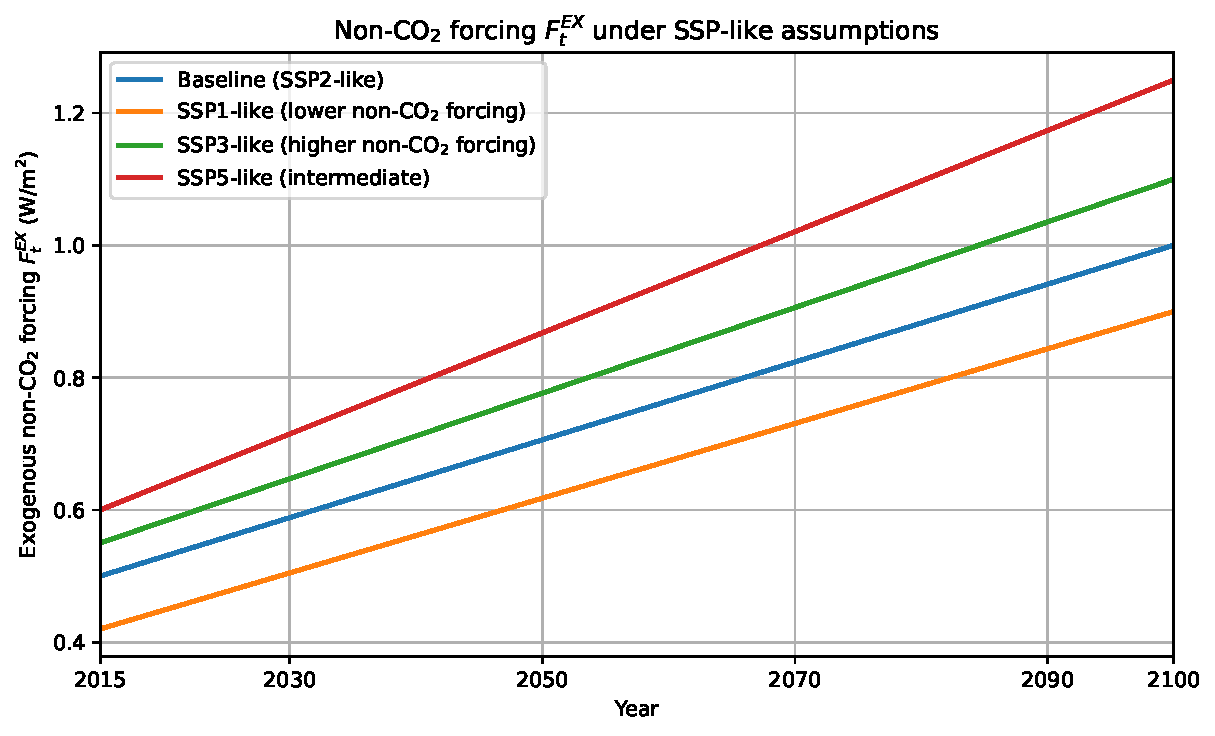
\includegraphics[width=0.6\textwidth]{images/figure_FEX.pdf}\newline
\end{center}

%

%TCIMACRO{\TeXButton{Transition: Box Out}{\transboxout}}%
%BeginExpansion
\transboxout
%EndExpansion%
%TCIMACRO{\TeXButton{EndFrame}{\end{frame}}}%
%BeginExpansion
\end{frame}%
%EndExpansion


\subsection{The socioeconomic block}%

%TCIMACRO{\TeXButton{BeginFrame}{\begin{frame}}}%
%BeginExpansion
\begin{frame}%
%EndExpansion
%

%TCIMACRO{\QTR{frametitle}{DICE: Input structure}}%
%BeginExpansion
\frametitle{DICE: Input structure}%
%EndExpansion


\begin{itemize}
\item World population (millions):
\begin{equation}
L_{t}=L_{t-\Delta}\left(  L_{\infty}/L_{t-\Delta}\right)  ^{\ell_{g}},
\end{equation}
$\ell_{g}\in\lbrack0,1]\hspace{0.1cm}${\normalsize convergence rate,
}$L_{\infty}\in\lbrack0,+\infty)\ ${\normalsize long term population.}%
%TCIMACRO{\TeXButton{vspace}{\vspace{4ex}}}%
%BeginExpansion
\vspace{4ex}%
%EndExpansion


\item Law of motion of capital:
\begin{equation}
K_{t}=\left(  1-\delta_{K}\right)  ^{\Delta}K_{t-\Delta}+I_{t},
\end{equation}
$\delta_{K}\in\lbrack0,1]$ is the depreciation rate{\normalsize , while
}$\Delta${\normalsize \ is the time step (here }$\Delta=5$ years)%
%TCIMACRO{\TeXButton{vspace}{\vspace{4ex}}}%
%BeginExpansion
\vspace{4ex}%
%EndExpansion

\end{itemize}

%

%TCIMACRO{\TeXButton{Transition: Box Out}{\transboxout}}%
%BeginExpansion
\transboxout
%EndExpansion%
%TCIMACRO{\TeXButton{EndFrame}{\end{frame}}}%
%BeginExpansion
\end{frame}%
%EndExpansion
%

%TCIMACRO{\TeXButton{BeginFrame}{\begin{frame}}}%
%BeginExpansion
\begin{frame}%
%EndExpansion
%

%TCIMACRO{\QTR{frametitle}{DICE:\ Example of population dynamics}}%
%BeginExpansion
\frametitle{DICE:\ Example of population dynamics}%
%EndExpansion


\begin{center}
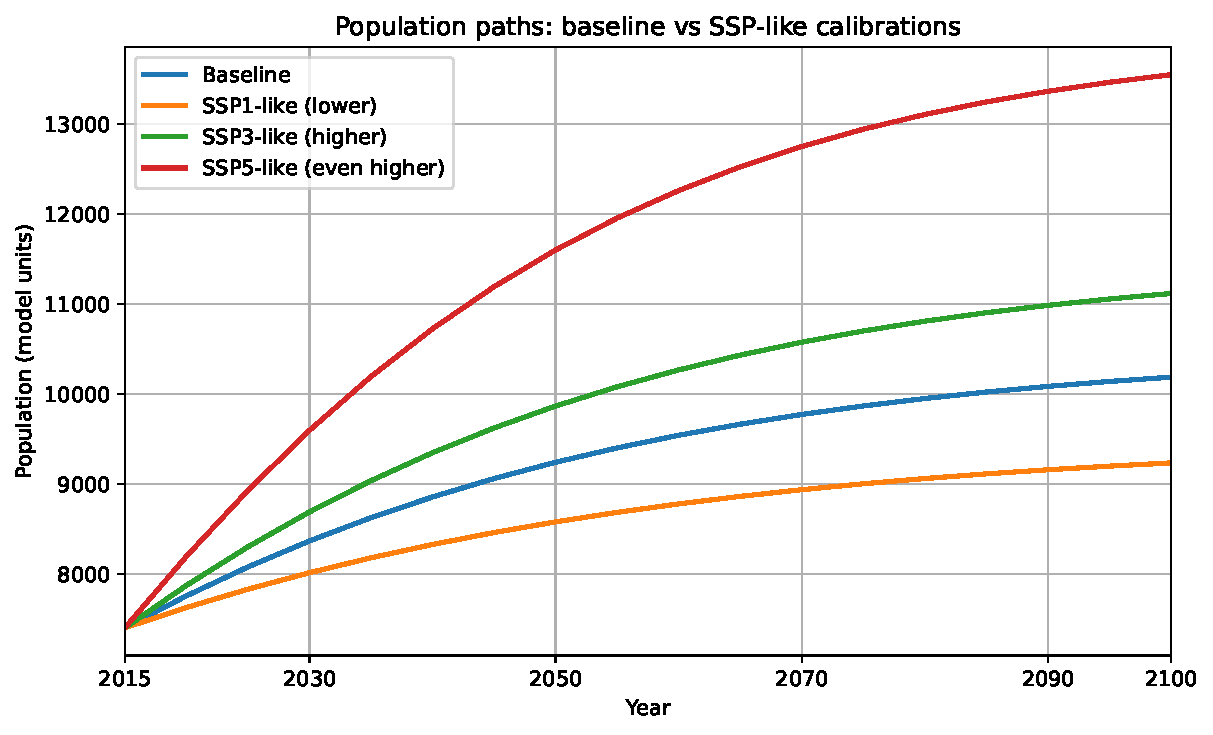
\includegraphics[width=0.6\textwidth]{images/figure_L.pdf}\newline
\end{center}

%

%TCIMACRO{\TeXButton{Transition: Box Out}{\transboxout}}%
%BeginExpansion
\transboxout
%EndExpansion%
%TCIMACRO{\TeXButton{EndFrame}{\end{frame}}}%
%BeginExpansion
\end{frame}%
%EndExpansion
%

%TCIMACRO{\TeXButton{BeginFrame}{\begin{frame}}}%
%BeginExpansion
\begin{frame}%
%EndExpansion
%

%TCIMACRO{\QTR{frametitle}{DICE: Production of goods}}%
%BeginExpansion
\frametitle{DICE: Production of goods}%
%EndExpansion


\begin{itemize}
\item Production is Cobb-Douglas in thousands USD:%
\begin{equation}
Y_{t}=A_{t}K_{t-\Delta}^{\gamma}\left(  \frac{L_{t}}{1,000}\right)
^{1-\gamma}%
\end{equation}
where $\gamma\in\lbrack0,1]$\ is capital intensity, physical capital
$K_{t-\Delta}$.%
%TCIMACRO{\TeXButton{vspace}{\vspace{4ex}}}%
%BeginExpansion
\vspace{4ex}%
%EndExpansion


\item Exogenous total productivity $A_{t}$ (with vanishing growth)%
\begin{equation}
A_{t}=A_{t-\Delta}/(1-g_{A}\exp(-\delta_{A}\left(  t-t_{0}\right)  ))
\end{equation}
$g_{A}\geq0$ the initial productivity growth and decay rate $\delta_{a}%
\in(0,1]$ to match declining productivity growth
\end{itemize}

%

%TCIMACRO{\TeXButton{Transition: Box Out}{\transboxout}}%
%BeginExpansion
\transboxout
%EndExpansion%
%TCIMACRO{\TeXButton{EndFrame}{\end{frame}}}%
%BeginExpansion
\end{frame}%
%EndExpansion
%

%TCIMACRO{\TeXButton{BeginFrame}{\begin{frame}}}%
%BeginExpansion
\begin{frame}%
%EndExpansion
%

%TCIMACRO{\QTR{frametitle}{DICE:\ Example of productivity dynamics}}%
%BeginExpansion
\frametitle{DICE:\ Example of productivity dynamics}%
%EndExpansion


\begin{center}
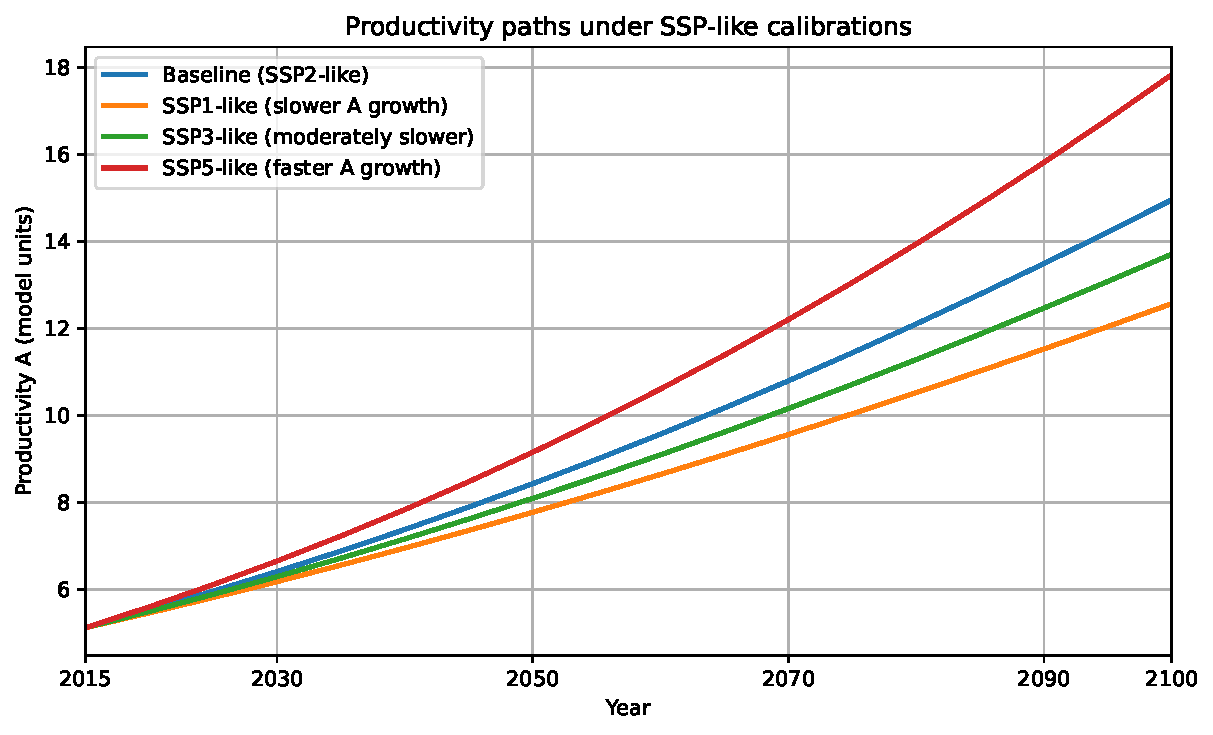
\includegraphics[width=0.8\textwidth]{images/figure_A.pdf}\newline
\end{center}

%

%TCIMACRO{\TeXButton{Transition: Box Out}{\transboxout}}%
%BeginExpansion
\transboxout
%EndExpansion%
%TCIMACRO{\TeXButton{EndFrame}{\end{frame}}}%
%BeginExpansion
\end{frame}%
%EndExpansion
%

%TCIMACRO{\TeXButton{BeginFrame}{\begin{frame}}}%
%BeginExpansion
\begin{frame}%
%EndExpansion
%

%TCIMACRO{\QTR{frametitle}{DICE: Emissions}}%
%BeginExpansion
\frametitle{DICE: Emissions}%
%EndExpansion


\begin{itemize}
\item Emissions (GtCO2):%
\begin{equation}
E_{t}=\Delta\cdot\left(  \sigma_{t}\left(  1-\mu_{t}\right)  Y_{t}%
+E_{t}^{\text{land}}\right)
\end{equation}
where $\sigma_{t}$\ decoupling rate, $\mu_{t}$\ is abatement share,
$E_{t}^{\text{land}}$ is exogenous process of carbon emission from change in
land use (i.e. deforestation, \ \symbol{126}10\%\ of emissions).%
%TCIMACRO{\TeXButton{vspace}{\vspace{4ex}}}%
%BeginExpansion
\vspace{4ex}%
%EndExpansion


\item Exogenous decoupling of emissions to GDP%
\begin{equation}
\sigma_{t}=\sigma_{t-\Delta}\exp\!\Big(-\,g_{\sigma}\,\big(1-\delta_{\sigma
}\big)^{\left(  t-t_{0}\right)  }\,\Delta\Big)
\end{equation}
$g_{\sigma}\geq0$ the initial decoupling rate and decay rate $\delta_{\sigma
}\in(0,1]$ to match emissions to GDP\ data.
\end{itemize}

%

%TCIMACRO{\TeXButton{Transition: Box Out}{\transboxout}}%
%BeginExpansion
\transboxout
%EndExpansion%
%TCIMACRO{\TeXButton{EndFrame}{\end{frame}}}%
%BeginExpansion
\end{frame}%
%EndExpansion
%

%TCIMACRO{\TeXButton{BeginFrame}{\begin{frame}}}%
%BeginExpansion
\begin{frame}%
%EndExpansion
%

%TCIMACRO{\QTR{frametitle}{DICE:\ Example of technology dynamics}}%
%BeginExpansion
\frametitle{DICE:\ Example of technology dynamics}%
%EndExpansion


\begin{center}
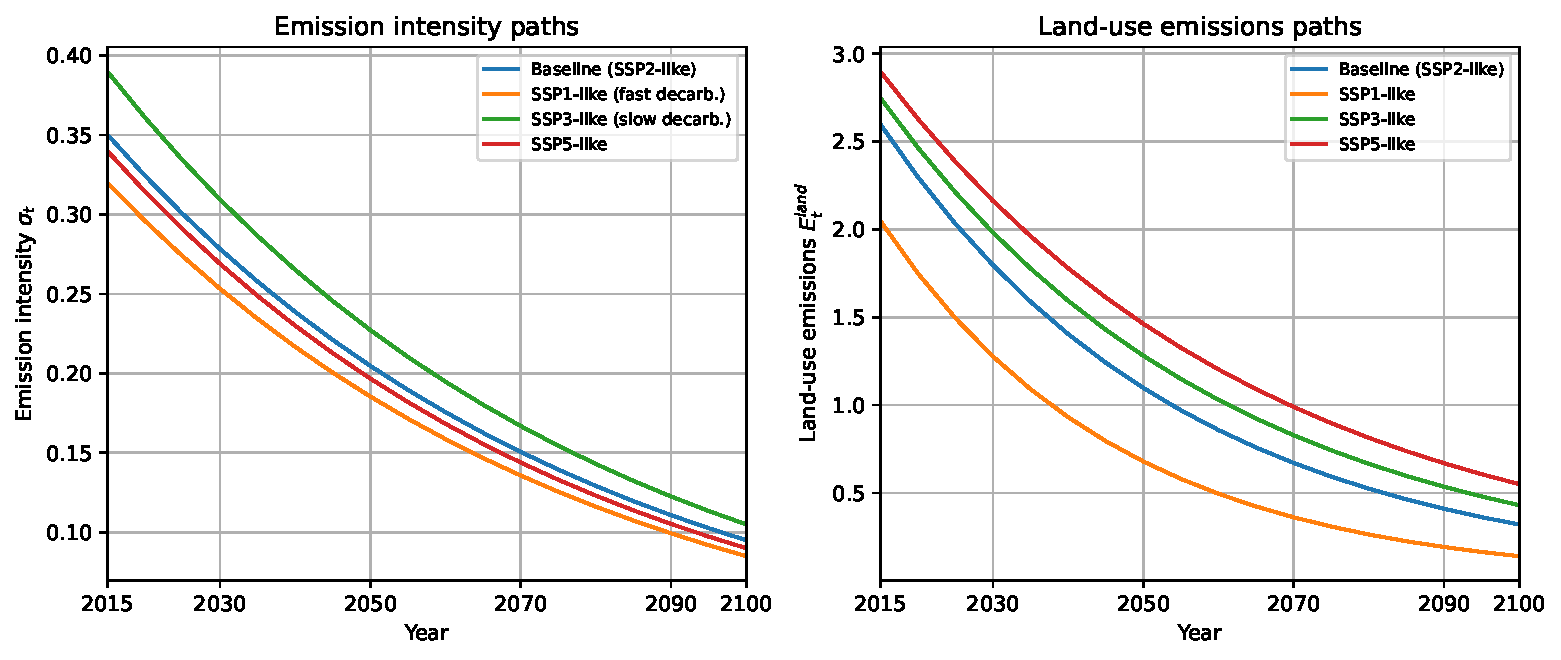
\includegraphics[width=0.8\textwidth]{images/figure_sigma_Eland.pdf}\newline
\end{center}

%

%TCIMACRO{\TeXButton{Transition: Box Out}{\transboxout}}%
%BeginExpansion
\transboxout
%EndExpansion%
%TCIMACRO{\TeXButton{EndFrame}{\end{frame}}}%
%BeginExpansion
\end{frame}%
%EndExpansion
%

%TCIMACRO{\TeXButton{BeginFrame}{\begin{frame}}}%
%BeginExpansion
\begin{frame}%
%EndExpansion
%

%TCIMACRO{\QTR{frametitle}{DICE: Equilibrium in goods and climate}}%
%BeginExpansion
\frametitle{DICE: Equilibrium in goods and climate}%
%EndExpansion


\begin{itemize}
\item Resource constraint:
\begin{equation}
Y_{t}\left(  1-\theta_{1,t}\mu_{t}^{\theta_{2}}\right)  \Omega\left(
T_{t-\Delta}^{AT}\right)  =C_{t}+I_{t}%
\end{equation}
LHS\ is output loss from abatement and damage, RHS is demand
side{\normalsize .}%
%TCIMACRO{\TeXButton{vspace}{\vspace{1ex}}}%
%BeginExpansion
\vspace{1ex}%
%EndExpansion


\item Damages are given by:%
\begin{equation}
\Omega\left(  T_{t-\Delta}^{AT}\right)  =1/(1+a\left(  T_{t-\Delta}%
^{AT}\right)  ^{2})
\end{equation}
This expression is subject to deep uncertainty, and should be taken as a
normative measure of the social loss for the society of rising temperatures.
Tipping points could be introduced [%
%TCIMACRO{\TeXButton{\citealp}{\citealp{weitzman2012ghg}}}%
%BeginExpansion
\citealp{weitzman2012ghg}%
%EndExpansion
].%
%TCIMACRO{\TeXButton{vspace}{\vspace{1ex}}}%
%BeginExpansion
\vspace{1ex}%
%EndExpansion


\item Abatement good technology decreases over time:%
\begin{equation}
\theta_{1,t}=\frac{p_{b}}{1000\,\theta_{2}}\,\big(1-\delta_{pb}\big)^{\left(
t-t_{0}\right)  }\,\sigma_{t}.
\end{equation}
where $p_{b}>0$ price of carbon to reach net zero, efficiency factor
$\delta_{pb}\in\lbrack0,1]$.
\end{itemize}

%

%TCIMACRO{\TeXButton{Transition: Box Out}{\transboxout}}%
%BeginExpansion
\transboxout
%EndExpansion%
%TCIMACRO{\TeXButton{EndFrame}{\end{frame}}}%
%BeginExpansion
\end{frame}%
%EndExpansion
%

%TCIMACRO{\TeXButton{BeginFrame}{\begin{frame}}}%
%BeginExpansion
\begin{frame}%
%EndExpansion
%

%TCIMACRO{\QTR{frametitle}{DICE:\ Example of abatement technology}}%
%BeginExpansion
\frametitle{DICE:\ Example of abatement technology}%
%EndExpansion


\begin{center}
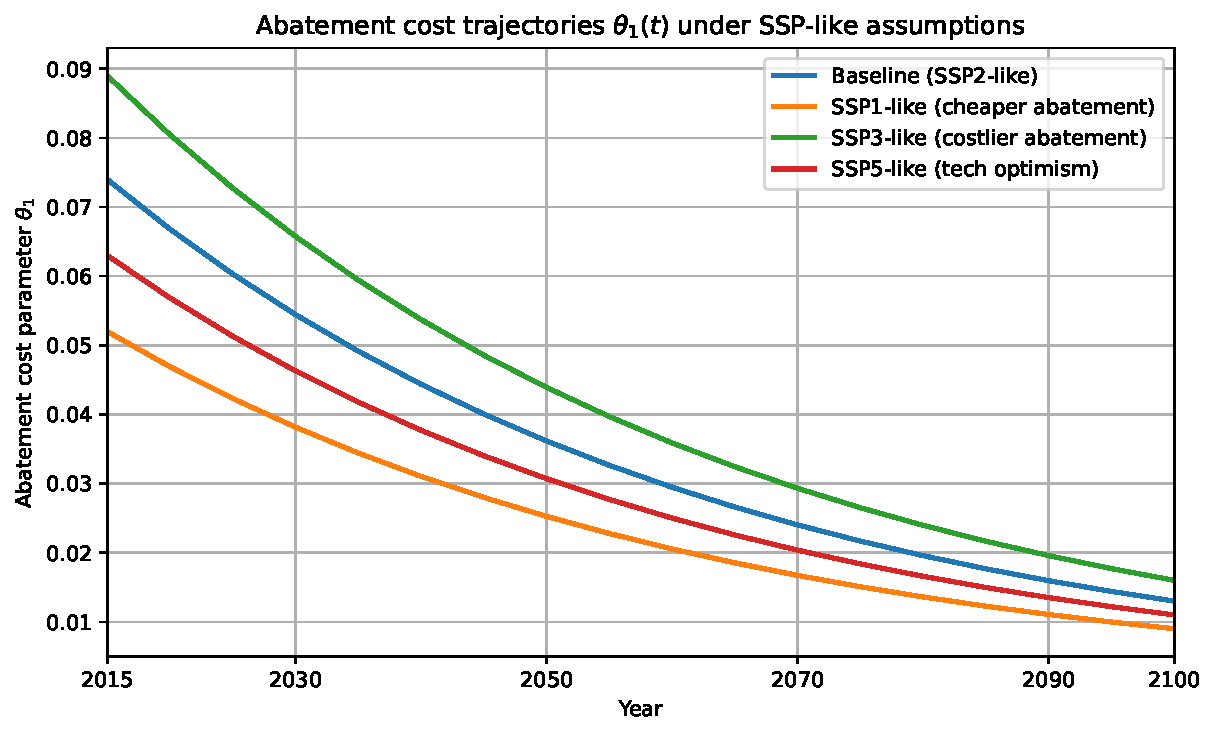
\includegraphics[width=0.8\textwidth]{images/figure_theta1.pdf}\newline
\end{center}

%

%TCIMACRO{\TeXButton{Transition: Box Out}{\transboxout}}%
%BeginExpansion
\transboxout
%EndExpansion%
%TCIMACRO{\TeXButton{EndFrame}{\end{frame}}}%
%BeginExpansion
\end{frame}%
%EndExpansion
%

%TCIMACRO{\TeXButton{BeginFrame}{\begin{frame}}}%
%BeginExpansion
\begin{frame}%
%EndExpansion


Total factor productivity:%
\[
A_{t}=A_{t-\Delta}/(1-g_{A}\exp(-\delta_{A}\left(  t-t_{0}\right)  ))
\]
Decoupling rate of carbon emission to GDP:%
\[
\sigma_{t}=\sigma_{t-\Delta}\exp\!\Big(-\,g_{\sigma}\,\big(1-\delta_{\sigma
}\big)^{\left(  t-t_{0}\right)  }\,\Delta\Big)
\]
Cost of abating carbon emissions:%
\[
\theta_{1,t}=\frac{p_{b}}{1000\,\theta_{2}}\,\big(1-\delta_{pb}\big)^{\left(
t-t_{0}\right)  }\,\sigma_{t}%
\]
Non-CO2 forcing law of motion:%
\[
F_{t}^{EX}=\min\left(  F_{t-\Delta}^{EX}+\Delta\cdot d_{F},F_{CAP}\right)
\]
Land-use law of motion:%
\[
E_{t}^{\text{land}}=\left(  1-\delta_{e}\right)  ^{\Delta}E_{t-\Delta
}^{\text{land}}%
\]
World population dynamic:%
\[
L_{t}=L_{t-\Delta}\left(  L_{T}/L_{t-\Delta}\right)  ^{\ell_{g}}%
\]
%

%TCIMACRO{\TeXButton{Transition: Box Out}{\transboxout}}%
%BeginExpansion
\transboxout
%EndExpansion%
%TCIMACRO{\TeXButton{EndFrame}{\end{frame}}}%
%BeginExpansion
\end{frame}%
%EndExpansion
%

%TCIMACRO{\TeXButton{BeginFrame}{\begin{frame}}}%
%BeginExpansion
\begin{frame}%
%EndExpansion


\begin{center}
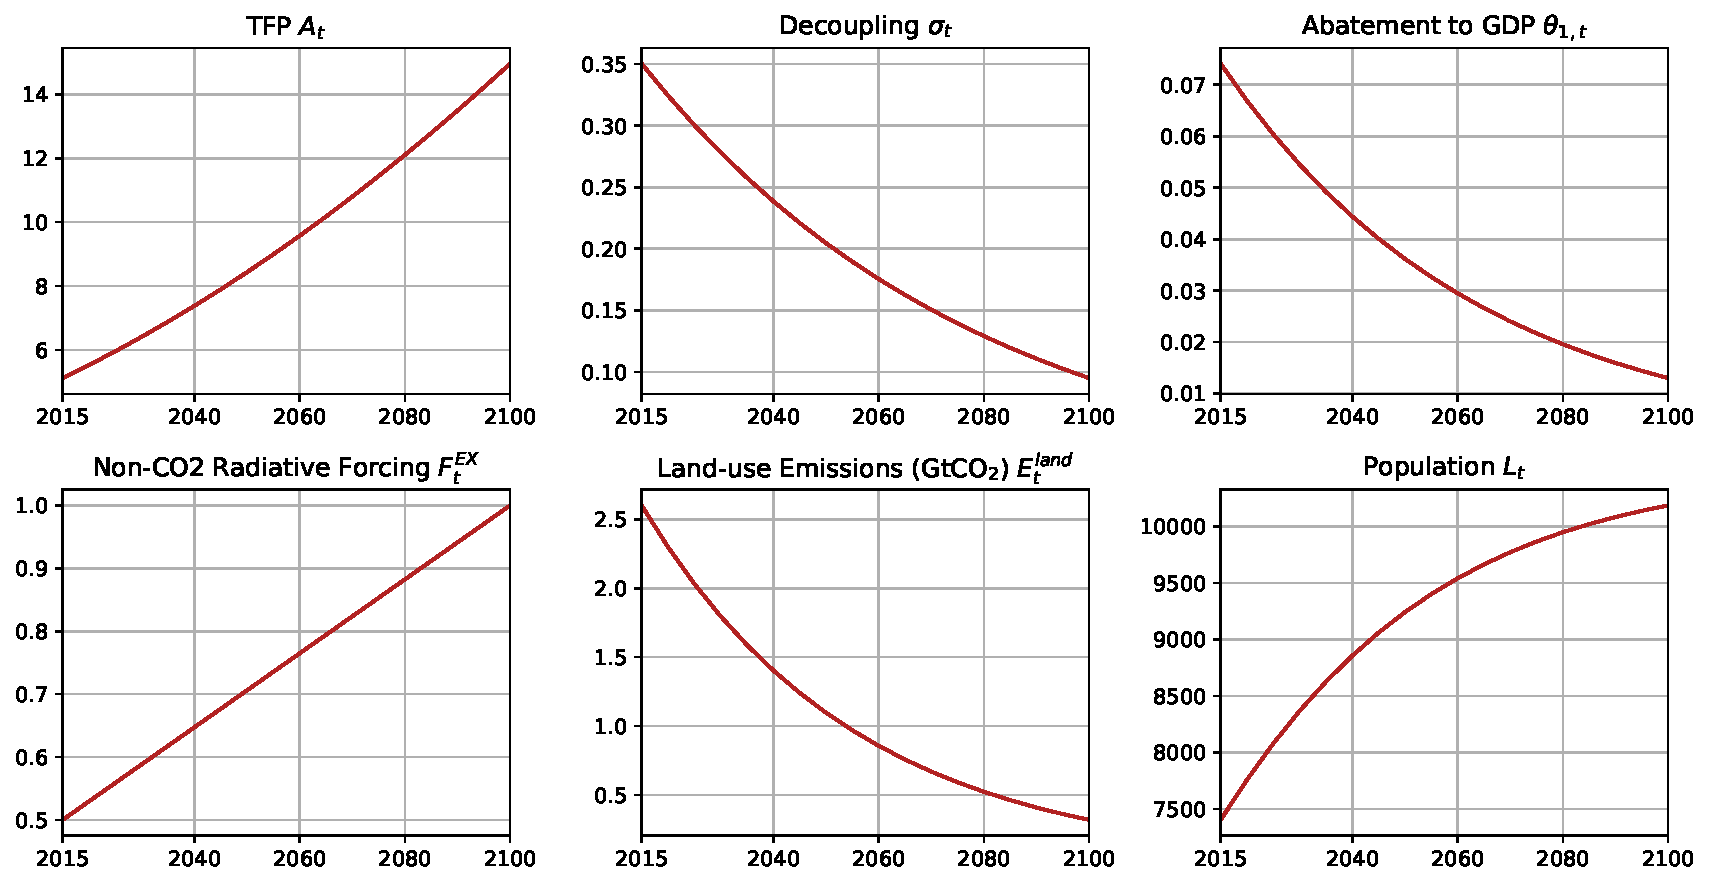
\includegraphics[width=0.88\textwidth]{images/figure_2.pdf}\newline

Figure.\ Summary of exogenous variables
\end{center}

%

%TCIMACRO{\TeXButton{Transition: Box Out}{\transboxout}}%
%BeginExpansion
\transboxout
%EndExpansion%
%TCIMACRO{\TeXButton{EndFrame}{\end{frame}}}%
%BeginExpansion
\end{frame}%
%EndExpansion


\subsection{Economic decisions}%

%TCIMACRO{\TeXButton{BeginFrame}{\begin{frame}}}%
%BeginExpansion
\begin{frame}%
%EndExpansion
%

%TCIMACRO{\QTR{frametitle}{DICE: Introducing a saving rate}}%
%BeginExpansion
\frametitle{DICE: Introducing a saving rate}%
%EndExpansion


\begin{itemize}
\item How should we determine optimally $C$ and $I$?%
%TCIMACRO{\TeXButton{vspace}{\vspace{1ex}}}%
%BeginExpansion
\vspace{1ex}%
%EndExpansion


\item We introduce optimal saving rate $s$, consumption and investment
becomes:%
\begin{align}
C_{t} &  =\Delta\cdot\left(  1-s_{t}\right)  \times Y_{t}\left(
1-\theta_{1,t}\mu_{t}^{\theta_{2}}\right)  \Omega\left(  T_{t-\Delta}%
^{AT}\right)  \\
I_{t} &  =\text{ \ \ \ \ \ \ \ \ \ }\Delta\cdot s_{t}\times Y_{t}\left(
1-\theta_{1,t}\mu_{t}^{\theta_{2}}\right)  \Omega\left(  T_{t-\Delta}%
^{AT}\right)
\end{align}
$\rightarrow$implicitely assuming that income spent between $C_{t}$ and
$I_{t}$.%
%TCIMACRO{\TeXButton{vspace}{\vspace{1ex}}}%
%BeginExpansion
\vspace{1ex}%
%EndExpansion


\item Here, $s$ is \textquotedblleft decision\textquotedblright\ variable,
which usually is pinned down by optimal control problem in economics.%
%TCIMACRO{\TeXButton{vspace}{\vspace{1ex}}}%
%BeginExpansion
\vspace{1ex}%
%EndExpansion

\end{itemize}

\begin{assumption}
[1]In what follows, we assume that $\{s_{t}\}_{t=t_{0}}^{T}=0.25$ as
simplifying assumption.
\end{assumption}

%

%TCIMACRO{\TeXButton{Transition: Box Out}{\transboxout}}%
%BeginExpansion
\transboxout
%EndExpansion%
%TCIMACRO{\TeXButton{EndFrame}{\end{frame}}}%
%BeginExpansion
\end{frame}%
%EndExpansion
%

%TCIMACRO{\TeXButton{BeginFrame}{\begin{frame}}}%
%BeginExpansion
\begin{frame}%
%EndExpansion
%

%TCIMACRO{\QTR{frametitle}{DICE: Introducing the abatement rate }}%
%BeginExpansion
\frametitle{DICE: Introducing the abatement rate }%
%EndExpansion


\begin{itemize}
\item Environmental policy here, denoted by abatement share $\mu_{t}$, is the
second decision variable.%
%TCIMACRO{\TeXButton{vspace}{\vspace{1ex}}}%
%BeginExpansion
\vspace{1ex}%
%EndExpansion


\item Increasing $\mu_{t}$\ has several economic and social implications:%
%TCIMACRO{\TeXButton{vspace}{\vspace{1ex}}}%
%BeginExpansion
\vspace{1ex}%
%EndExpansion


\begin{itemize}
\item $\partial C_{t}/\partial\mu_{t}<0$ : $\mu_{t}\nearrow$ crowds out
\textbf{consumption}.\ Yellow vest effect which can threaten the
implementation of the policy.%
%TCIMACRO{\TeXButton{vspace}{\vspace{1ex}}}%
%BeginExpansion
\vspace{1ex}%
%EndExpansion


\item $\partial I_{t}/\partial\mu_{t}<0$ : $\mu_{t}\nearrow$ crowds out
\textbf{investment}.\ Lower growth prospects in the future.%
%TCIMACRO{\TeXButton{vspace}{\vspace{1ex}}}%
%BeginExpansion
\vspace{1ex}%
%EndExpansion


\item $\partial E_{t}/\partial\mu_{t}<0$ : $\mu_{t}\nearrow$ reduces carbon
emissions.%
%TCIMACRO{\TeXButton{vspace}{\vspace{1ex}}}%
%BeginExpansion
\vspace{1ex}%
%EndExpansion

\end{itemize}
\end{itemize}

\begin{assumption}
[2]In what follows, we will give as an input (exogenously) the sequence
$\{\mu_{t}\}_{t=t_{0}}^{T}$ of abatement.
\end{assumption}

%

%TCIMACRO{\TeXButton{Transition: Box Out}{\transboxout}}%
%BeginExpansion
\transboxout
%EndExpansion%
%TCIMACRO{\TeXButton{EndFrame}{\end{frame}}}%
%BeginExpansion
\end{frame}%
%EndExpansion
%

%TCIMACRO{\TeXButton{BeginFrame}{\begin{frame}}}%
%BeginExpansion
\begin{frame}%
%EndExpansion
%

%TCIMACRO{\QTR{frametitle}{DICE: model summary}}%
%BeginExpansion
\frametitle{DICE: model summary}%
%EndExpansion


\begin{itemize}
\item \textbf{Exogenous variables} each driven by an exogenous process
(growth/decline path).%
\[
x_{t}=\{A_{t},\ \sigma_{t},\ \theta_{1,t},\ F_{t}^{EX},\ E_{t}^{\text{land}%
},\ L_{t}\}
\]


\item \textbf{Endogenous state/flow variables}%
\[
y_{t}=\{M_{t}^{AT},\ M_{t}^{UP},\ M_{t}^{LO},\ T_{t}^{AT},\ T_{t}^{LO}%
,\ Y_{t},\ K_{t},\ C_{t}\}
\]


\item \textbf{Decision variables (or controls)}%
\[
z_{t}=\{\mu_{t},\ s_{t}\}
\]


\item \textbf{Horizon and time step:} $t\in\{2015,2020,2025,\ldots,T\}$,
$\Delta=5$ years (quinqennial).
\end{itemize}

%

%TCIMACRO{\TeXButton{Transition: Box Out}{\transboxout}}%
%BeginExpansion
\transboxout
%EndExpansion%
%TCIMACRO{\TeXButton{EndFrame}{\end{frame}}}%
%BeginExpansion
\end{frame}%
%EndExpansion
%

%TCIMACRO{\TeXButton{BeginFrame}{\begin{frame}}}%
%BeginExpansion
\begin{frame}%
%EndExpansion
%

%TCIMACRO{\QTR{frametitle}{DICE: A sketch of the numerical solution}}%
%BeginExpansion
\frametitle{DICE: A sketch of the numerical solution}%
%EndExpansion


Under Assumptions (1) and (2), the numerical solution is straightforward
through an open loop:
\begin{align*}
x_{t}  &  =g(x_{t-1}),\qquad\text{\ \ \ \ \ \ \ \ \ }g:\ \mathbb{R}^{N_{x}%
}\rightarrow\mathbb{R}^{N_{x}},\\[0.3em]
y_{t}  &  =f\big(y_{t-1},\,x_{t},\,z_{t}\big),\qquad f:\ \mathbb{R}^{N_{y}%
}\times\mathbb{R}^{N_{x}}\times\mathbb{R}^{2}\rightarrow\mathbb{R}^{N_{y}}.
\end{align*}


\begin{itemize}
\item $x_{t}\in\mathbb{R}^{N_{x}}$: \textbf{exogenous variables}
($A_{t},\ \sigma_{t},\ \ldots, L_{t}$).

\item $y_{t}\in\mathbb{R}^{N_{y}}$: \textbf{endogenous states/flows}
($M_{t}^{AT},M_{t}^{UP},\ldots,Y_{t},K_{t}$).

\item $z_{t}=[\mu_{t},s_{t}]^{\prime}\in\mathbb{R}^{2}$: \textbf{decision
variables} (abatement, saving).
\end{itemize}

%

%TCIMACRO{\TeXButton{Transition: Box Out}{\transboxout}}%
%BeginExpansion
\transboxout
%EndExpansion%
%TCIMACRO{\TeXButton{EndFrame}{\end{frame}}}%
%BeginExpansion
\end{frame}%
%EndExpansion
%

%TCIMACRO{\TeXButton{BeginFrame}{\begin{frame}}}%
%BeginExpansion
\begin{frame}%
%EndExpansion


\begin{center}
Thank you!

\vspace{5ex}

$\mathtt{gauthier.vermandel@polytechnique.edu}$
\end{center}

%

%TCIMACRO{\TeXButton{Transition: Box Out}{\transboxout}}%
%BeginExpansion
\transboxout
%EndExpansion%
%TCIMACRO{\TeXButton{EndFrame}{\end{frame}}}%
%BeginExpansion
\end{frame}%
%EndExpansion
%

%TCIMACRO{\TeXButton{FRAME}{\bibliographystyle{apalike}
%\bibliography{lucas_romie}}}%
%BeginExpansion
\bibliographystyle{apalike}
\bibliography{lucas_romie}%
%EndExpansion



\end{document}
